\chapter{Distributed MPC for Formation Path-Following of Multi-Vehicle Systems}
\label{chap:handpos_MPC}

\pgfplotsset{table/search path={figures/handpos_MPC/data}}

The chapter considers the problem of formation path-following of multiple vehicles and proposes a solution based on combining distributed model predictive control with parametrizations of the trajectories of the vehicles using polynomial splines. Introducing such parametrization leads indeed to two potential benefits: a) reducing the number of optimization variables, and b) enabling enforcing constraints on the vehicles in a computationally efficient way. Moreover, the proposed solution formulates the formation path-following problem as a distributed optimization problem that may then be solved using the \gls{admm}.
The proposed approach is applicable to all vehicles that can be modeled as differentially flat systems.
In this chapter, we present numerical simulations with \acrlongpl{auv} and differential drive robots.
The contents of this chapter are based on \cite{matous_MPC_2022}.

The chapter is organized as follows.
In Section~\ref{sec:MPC_problem-description}, we present the general assumptions on the model of the vehicles and formally define the formation path-following problem.
In Section~\ref{sec:MPC_spline-based-MPC}, we propose the distributed spline-based \gls{mpc} scheme.
Finally, Section~\ref{sec:MPC_case_studies} presents two numerical case studies.

\section{Problem Description}
\label{sec:MPC_problem-description}

In this section, we first introduce the assumptions on the model of the vehicles.
Then, we define the objective of formation path-following and pose it as an optimization problem.



\subsection{Vehicle Model}
\label{ssec:MPC_vehicle-model}

\dt{As mentioned in the introduction to this chapter, the proposed \gls{mpc} algorithm can be applied to a wide range of vehicles, not just \glspl{auv}.
Consequently, the model presented in this section is more general than the hand position model presented in Chapter~\ref{chap:handpos_definition}.
A case study showing how the theory developed in this chapter can be applied to \glspl{auv} will be presented in Section~\ref{sec:MPC_case_study_AUV}.}

Here, we discuss the dynamics of a single agent in the network. Let $\mat{x} \in \mathbb{R}^{n_{\mat{x}}}$ be the vector of states.
We assume that the state vector includes the position of the agent.
Without loss of generality, let the first $n_{\mat{q}}$ states be the position of the vehicle.
We can then define the position vector of the vehicle as
\begin{equation}
    \mat{q} = \inlinevector{x_1, \ldots, x_{n_{\mat{q}}}}.
\end{equation}
Since vehicles typically move in either two or three dimensions, we assume that $n_{\mat{q}} \in \left\{2,3\right\}$.
Let $\mat{u} \in \mathbb{R}^{n_{\mat{q}}}$ be the vector of control inputs.
We assume the dynamics of the vehicle to be given by an ordinary differential equation
\begin{equation}
    \dot{\mat{x}} = f \left(\mat{x}, \mat{u}\right).
\label{equ:MPC_dynamics-of-an-agent}
\end{equation}
%where $f : \mathbb{R}^{n_{\mat{x}}} \times \mathbb{R}^{n_{\mat{q}}} \mapsto \mathbb{R}^{n_{\mat{x}}}$ 
Note that we assume the number of inputs to be equal to $n_{\mat{q}}$.
In cases where this assumption does not hold because the vehicle is overactuated, we need to reduce the number of inputs by introducing a control allocation scheme (see, \emph{e.g.,} \cite{johansen_control_2013}).

Let $\mat{y} \in \mathbb{R}^{n_{\mat{q}}}$ be the output of the system.
Note that, in general, the output can be different from the position of the vehicle.
However, as discussed in the next paragraph, it must be possible to obtain the position from the output.

We assume the system to be differentially flat \cite{fliess_1995_flatness}, \emph{i.e.}, we assume that the input and state can be determined from the output, its derivatives, and antiderivatives. Moreover, we assume that the relation between the output and the position is polynomial.
In other words, there exist suitable (nonlinear) functions $\bm{\phi}_{\mat{u}}$ and $\bm{\phi}_{\mat{x}}$, and a multidimensional polynomial function $\bm{\phi}_{\mat{q}}$ of suitable dimensions such that, at any time,
%
\begin{align}
    \mat{u} &= \bm{\phi}_{\mat{u}} \left(\mat{y}, \dot{\mat{y}}, \ddot{\mat{y}}, \ldots, \mat{y}^{(r')}\right), \label{eq:MPC_phi_u} \\
    \mat{x} &= \bm{\phi}_{\mat{x}} \left(\mat{y}^{(-r'')}, \ldots, \mat{y}, \dot{\mat{y}}, \ddot{\mat{y}}, \ldots, \mat{y}^{(r')}\right), \label{eq:MPC_phi_x} \\ 
    \mat{q} &= \bm{\phi}_{\mat{q}} \left(\mat{y}^{(-r'')}, \ldots, \mat{y}, \dot{\mat{y}}, \ddot{\mat{y}}, \ldots, \mat{y}^{(r')}\right), \label{eq:MPC_phi_q}
\end{align}
%
where $r'$ and $r''$ are positive integers.

To model the constraints on the dynamics of the vehicle, we use a multidimensional function $\mat{e}$.
The set of feasible states and inputs is given by
\begin{equation}
    \big\{\left(\mat{x}, \mat{u}\right) \big| \mat{e} (\mat{x}, \mat{u}) \geq \bm{0}\big\}
    \label{eq:MPC_e}
\end{equation}
where the inequality is defined component-wise.
We assume that substituting \eqref{eq:MPC_phi_u}, \eqref{eq:MPC_phi_x} into \eqref{eq:MPC_e} yields a set of polynomial constraints.
In other words, we assume that there exists a multidimensional polynomial function $\mat{h}$ such that
\begin{equation}
    \mat{e} (\mat{x}, \mat{u})
    \geq
    \bm{0}
    \, \iff \,
    \mat{h} \left( \mat{y}^{(-r'')}, \ldots, \mat{y}^{(r')} \right)
    \geq
    \bm{0}.
\label{equ:MPC_constraint-h-geq-0}
\end{equation}



\subsection{Formation Path-Following Problem}
\label{ssec:MPC_formation-path-following}



The goal is to control $N$ vehicles, all subject to the dynamics introduced in Section~\ref{ssec:MPC_vehicle-model}, so that they move in a prescribed formation while their barycenter follows a given path.
Let $\mat{p}_p : \mathbb{R} \rightarrow \mathbb{R}^{n_{\mat{q}}}$ be a parametrization by arc length that is continuously differentiable.
This implies that for every path point $\mat{p}(s)$, we can define a path-tangential coordinate frame and a corresponding rotation matrix $\mat{R}_p(s)$ between the inertial and path-tangential frames (see Section~\ref{sec:background_paths}).

The vehicles should converge to a dynamic formation that rotates with the desired path (see Section~\ref{sec:background_formation_keeping}).
Let $\mat{p}_{f, 1}^f, \ldots, \mat{p}_{f, N}^f$ be the position vectors that represent the desired formation.
Using this notation, the desired trajectory for agent $i$ is given by
\begin{equation}
    \mat{q}_{d,i}(s) = \mat{p}_p(s) + \mat{R}_p(s)\, \mat{p}_{f, i}^f,
\end{equation} 
for a given $s$.

The objective of the control system is to steer the actual vehicle positions $\mat{q}_i(t)$ to follow the desired trajectories $\mat{q}_{d,i}$. Ideally, this means that for a given function $s(t)$ we seek the actual positions to be such that
\begin{equation}
    \mat{q}_i(t)
    \rightarrow
    \mat{q}_{d,i}\big(s(t)\big),
    \quad \forall i = 1, \ldots, N.
    \label{eq:MPC_path_goal}
\end{equation} 

Similarly to the \gls{nsb} algorithms in Part~\ref{part:NSB}, the path parameter $s(t)$ can be treated as an additional \emph{degree of freedom} when designing the controller. Consequently, we also need to find a suitable control law for $s(t)$. For this purpose, let $U_d$ be the desired speed of the barycenter of the formation. %It is then possible to use~\eqref{eq:MPC_path_assumption} to connect the desired speed of such barycenter with the actual speed of the actual barycenter $U(t)$ by means of
If the vehicles follow the path perfectly, the actual speed of the barycenter is given by
\begin{equation}
    U(t)
    =
    \norm{\dot{\mat{p}}_p \big( s(t) \big)}
    =
    \norm{\frac{\partial \mat{p}_p(s)}{\partial s}\,\dot{s}(t) } = \abs{\dot{s}(t)}.
\end{equation}
The equivalence above implies that the path parameter $s(t)$ should thus be chosen such that
\begin{equation}
    \dot{s} \rightarrow U_d.
    \label{eq:MPC_param_goal}
\end{equation}



\subsection{A Centralized Solution}
\label{ssec:MPC_centralized}



The problem of finding for each agent $i$ its actuation signal $\mat{u}_i(t)$ that guarantees following the desired path $\mat{q}_{d,i} \big( s(t) \big)$ as close as possible can thanks to~\eqref{eq:MPC_phi_u}--\eqref{eq:MPC_phi_q} be transformed into the problem of finding a corresponding output trajectory $\mat{y}_i(t)$.

In general, it is not possible to find an output trajectory $\mat{y}_i(t)$ such that \eqref{eq:MPC_path_goal} is satisfied, since the dynamics of the agents are constrained by both~\eqref{equ:MPC_dynamics-of-an-agent} and~\eqref{equ:MPC_constraint-h-geq-0}. This means that at any time $t$, there is a position error
%
\begin{equation}
    \widetilde{\mat{q}}_i(t)
    =
    \mat{q}_i(t)
    -
    \mat{q}_{d,i} \big( s(t) \big) .
    \label{eq:MPC_q_tilde}
\end{equation}
%
Thanks to \eqref{eq:MPC_phi_q}, we can express $\widetilde{\mat{q}}_i(t)$ in terms of $\mat{y}_i(t)$
\begin{equation}
    \widetilde{\mat{q}}_i(t)
    =
    \bm{\phi}_{\mat{q}}\left(\mat{y}^{(-r'')}(t), \ldots, \mat{y}^{(r')}(t)\right)
    -
    \mat{q}_{d,i} \big( s(t) \big), \label{eq:MPC_y_tilde}
\end{equation}
and thus solve the problem by optimizing $\mat{y}_i(t)$ and $s(t)$.

The problem should be cast in a receding horizon fashion to reject potential disturbances as the mission proceeds.     
We thus propose to formulate the \emph{centralized} problem of optimizing a part of the trajectory, i.e., $\{\mat{y}_i(t:t+T)\}$, $s(t:t+T)$, as that of solving the following constrained problem
%
\begin{equation}
    \begin{split}
        \opt_{ \left\lbrace \mat{y}_i(t:t+T) \right\rbrace, s(t:t+T)}
        \sum_{i=1}^N
        &
        \int_{t}^{t+T}
        \widetilde{\mat{q}}_i\T(\tau) \, \bm{Q}_{\mat{p}} \, \widetilde{\mat{q}}_i(\tau) {\rm d}\tau \\
        & 
        +
        \int_{t}^{t+T} Q_s\,\left(\dot{s}(\tau) - U_d\right)^2 {\rm d}\tau, 
    \end{split}
\label{eq:MPC_optimization_centralized}
\end{equation}
with $T$ being the prediction horizon, $\bm{Q}_{\mat{p}}$ and $Q_s$ positive weight matrices, $\dm{\widetilde{\mat{q}}_{i}}$ the position error as defined in~\eqref{eq:MPC_y_tilde}, and subject to, for every agent $i = 1, \ldots, N$, to the constraints~\ref{constraint:io} to~\ref{constraint:initial-condition} below:
\begin{enumerate}[label=C\arabic*]
    \item the implicit constraint on the inputs and states, \emph{i.e.}, $$\mat{h} \left( \mat{y}_i^{(-r'')}(\tau), \ldots, \mat{y}^{(r')}_i(\tau) \right) \geq \bm{0}, \quad \forall \tau \in [t, t + T],$$
    \label{constraint:io}
    \item the constraint on the initial condition of the state of the system, i.e., $$\bm{\phi}_{\mat{x}} \left(\mat{y}_i^{(-r'')}(t), \ldots, \mat{y}^{(r')}_i(t)\right) = \mat{x}_{i}(t),$$
    \item the constraint on the initial condition of the path of the agents, \emph{i.e.}, $s(t)$. In other words, $s(t)$ is not a decision variable, while $s(t+\tau)$ for any $\tau > 0$ is.
    \label{constraint:initial-condition}
\end{enumerate}
We note that the variational problem above may not be solvable using off-the-shelf hardware with limited computing power. For this reason, it will be rewritten below.



\subsection{A Distributed Solution}

\da{To make the centralized approach from the previous section distributed, we assume \emph{synchronous bidirectional reliable} communication.
In other words, we assume that all vehicles exchange information simultaneously and there are no packet losses.
Bidirectional communication implies that the communication network can be described by an undirected graph $\mathcal{G} = \left(\mathcal{V}, \mathcal{E}\right)$, where $\mathcal{V} = \left\{1, \ldots, N\right\}$ correspond to the agents, and $\mathcal{E} \subseteq \mathcal{V} \times \mathcal{V}$ represents the communication between pairs of agents. We further assume that $\mathcal{G}$ is connected.
Similarly to Chapter~\ref{chap:distr_NSB}, we denote the set of neighbors of agent $i$ as $\mathcal{N}_i$.}

Before doing the rewriting, we note that it is possible to make \eqref{eq:MPC_optimization_centralized} distributed by letting the path parameter $s(t)$ be a local variable (\emph{i.e.}, $s_i(t)$), and adding a synchronization constraint on the set of $s_i(t)$'s. This leads to the local reformulation

\begin{subequations}
    \begin{align}
        \begin{split}
            &\opt_{ \left\lbrace \mat{y}_i(t:t+T), s_i(t:t+T) \right\rbrace }
            \int_{t}^{t+T}
                \widetilde{\mat{q}}_i\T(\tau)
                \, \bm{Q}_{\mat{p}} \, 
                \widetilde{\mat{q}}_i(\tau)
                {\rm d}\tau \\
            & \qquad \qquad \qquad \qquad
            + \int_{t}^{t+T} Q_s \,\left(\dot{s}_i(\tau) - U_d\right)^2 {\rm d}\tau , 
        \end{split} \label{eq:MPC_criterion}\\
        & \text{subject to } \, h\left(\mat{y}_i^{(-r'')}(\tau), \ldots, \mat{y}^{(r')}_i(\tau)\right) \geq \bm{0}, \label{eq:MPC_constraint_h} \\
        & \phantom{\text{subject to } \,} \bm{\phi}_{\mat{x}} \left(\mat{y}_i^{(-r'')}(t), \ldots, \mat{y}^{(r')}_i(t)\right) = \mat{x}_{i}(t), \label{eq:MPC_constraint_x0} \\
        & \phantom{\text{subject to } \,} s_i(\tau) = s_j(\tau), \quad \dm{\forall i \in \mathcal{V}, \forall j \in \mathcal{N}_i, \forall \tau \in [t, t+T]} \label{eq:MPC_constraint_gamma_s}
    \end{align}
\label{eq:MPC_optimization_distributed}

\end{subequations}

\noindent where $j$ is the index of the generic neighbor of agent $i$. This formulation is again only an intermediate step towards the approach proposed in this chapter, as explained below. 



\section{A Distributed Spline-Based MPC Solution}
\label{sec:MPC_spline-based-MPC}



The goal of this section is to show how constraining $\mat{y}_i$ and $s_i$ to be splines enables rewriting the variational problem above in a way that is computationally tractable.

For the sake of readability, we will use the convention for which sans-serif fonts (\emph{e.g.}, $\coefm{y}$) indicate quantities relative to splines, while serif fonts (\emph{e.g.}, $\mat{y}$) indicate trajectories parametrized in time as above. %Moreover, without loss of generality we assume $t = 0$, so that the to-be-designed trajectory is $\mat{y}_i(0:T)$.



\subsection{Spline Parametrization}
\label{ssec:MPC_spline_param}



Let $\coefm{b} = \inlinevector{\coef{b}_1, \ldots, \coef{b}_n}$ be the vector of basis functions of a B-spline, and let $\coefm{y}_i = \inlinevector{\coefm{y}_{i,1}\T, \ldots, \coefm{y}_{i,n}\T}$ be a generic matrix and $\coefm{s}_i = \inlinevector{\coef{s}_{i,1}, \ldots, \coef{s}_{i,n}}$ a generic vector of spline coefficients. Assume then that the trajectories and path parameters may be expressed as B-splines, i.e., as
%
\begin{align}
    \mat{y}_i(\tau) &= \sum_{l=1}^n \coefm{y}_{i,l}\,\coef{b}_l(\tau) = \coefm{y}_i\T\,\coefm{b}(\tau), \\
    s_i(\tau) &= \sum_{l=1}^n \coef{s}_{i,l}\,\coef{b}_l(\tau) = \coefm{s}_i\T\,\coefm{b}(\tau).
\end{align}
%
This assumption implies the possibility of exploiting the convex hull property
\begin{equation}
    \coefm{y}_i \geq \bm{0} \, \implies \, \mat{y}(\tau) \geq \bm{0},
\end{equation}
that implies that any polynomial constraint on a spline can be replaced by a (stricter) constraint on the spline coefficients.
In other words, by assuming the output to be a spline, we assume that there exists a function $\mathsf{h}$ such that
\begin{equation}
    \mathsf{h}\left(\coefm{y}_i\right) \geq \bm{0}
    \, \implies \,
    h\left(\mat{y}_i^{(-r'')}(\tau), \ldots, \mat{y}^{(r')}_i(\tau)\right) \geq \bm{0}.
\end{equation}

This eventually enables us to rewrite the trajectory optimization problems in Section~\ref{sec:MPC_problem-description} as corresponding spline-based \gls{mpc} problems. %In more details,   

%First, we need to locally approximate the path function and the associated rotation matrix using polynomials
To do so, each agent $i$ must locally approximate the path function and the associated rotation matrix as polynomials
\begin{align}
    \mat{p}_p(s) &\approx \mat{p}_{p, 0} + \mat{p}_{p, 1}\,s + \ldots + \mat{p}_{p, m}\,s^m, \\
    \mat{R}_p(s) &\approx \mat{R}_{p,0} + \mat{R}_{p,1}\,s + \ldots + \mat{R}_{p,m}\,s^m,
\end{align}
over an interval $\left[s_i(t), s_i(t) + s_T\right]$, where $t$ is the current time and $s_T$ is chosen such that $s_T \geq U_d T$.
We then need to impose an additional constraint on the path parameter
\begin{equation}
    s_i(t) \leq s_i(\tau) \leq s_i(t) + s_T, \quad \forall \tau \in \left[t, t + T\right], \label{eq:MPC_constraint_s_range}
\end{equation}
to ensure that the polynomial approximation is valid.

This approximation transforms the criterion from \eqref{eq:MPC_criterion} into a polynomial function.
The optimization problem \eqref{eq:MPC_optimization_distributed} can then be reformulated in terms of spline coefficients 
\begin{subequations}
    \begin{align}
            \opt_{\coefm{y}_i, \coefm{s}_i} &\, J_i\left(\coefm{y}_i, \coefm{s}_i\right), \\
        \text{subject to } & \coefm{y}_i \in \coef{Y}_i, \\
        & \coefm{s}_i \in \coef{S}_i, \\
        & \coefm{s}_i = \coefm{s}_j, \quad \dm{\forall i \in \mathcal{V}, \forall j \in \mathcal{N}_i}, \label{eq:MPC_s_constraint}
    \end{align} \label{eq:MPC_optimization_spline} 
\end{subequations}
\vspace*{-1em}

\noindent where $J_i$ is the objective function from \eqref{eq:MPC_criterion}, reformulated using the spline coefficients, and $\coef{Y}_i$ and $\coef{S}_i$ are the sets of feasible coefficients given by \eqref{eq:MPC_constraint_h}, \eqref{eq:MPC_constraint_x0} and \eqref{eq:MPC_constraint_s_range}.

This optimization problem is then solved in discrete time-steps.
Similarly to collocation-based \gls{mpc}, we can use the results from the previous time-step to ``warm-start'' the optimization problem.
We do this by extrapolating the previous results over the new horizon (see \figref{fig:MPC_warm_start}).

\begin{figure}[t]
    \centering
    % This file was created by matlab2tikz.
%
%The latest updates can be retrieved from
%  http://www.mathworks.com/matlabcentral/fileexchange/22022-matlab2tikz-matlab2tikz
%where you can also make suggestions and rate matlab2tikz.
%
\definecolor{mycolor1}{rgb}{0.00000,0.44700,0.74100}%
%
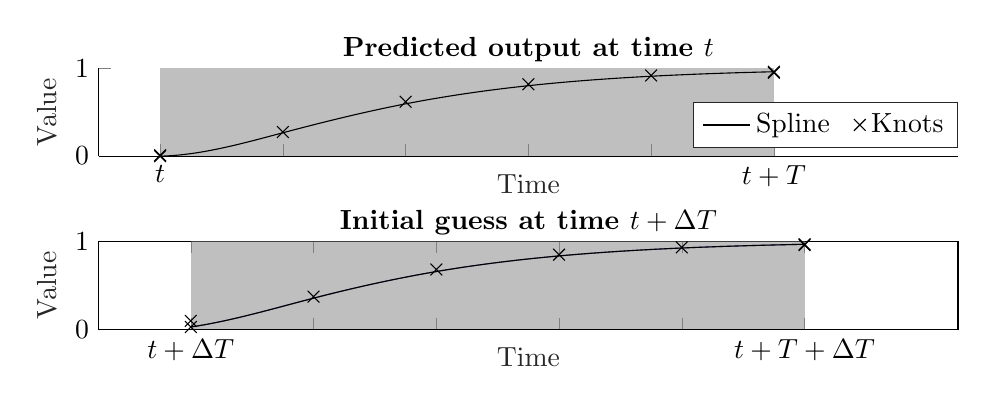
\begin{tikzpicture}

\begin{axis}[%
width=0.9\columnwidth,
height=11.176mm,
at={(0mm,22mm)},
scale only axis,
xmin=-0.5,
xmax=6.5,
xtick={0,1,2,3,4,5},
xticklabels={{$t$},{},{},{},{},{$t+T$}},
xlabel style={font=\color{white!15!black}, yshift=4mm},
xlabel={Time},
ymin=-0.00166163979628464,
ymax=1,
ytick={0,1},
ylabel style={font=\color{white!15!black}},
ylabel={Value},
axis background/.style={fill=white},
title style={font=\bfseries, yshift=-2.5mm},
title={Predicted output at time $t$},
axis x line*=bottom,
axis y line*=left,
legend style={at={(1,0.09)}, anchor=south east, legend cell align=left, align=left, draw=white!15!black},
legend columns=2
]

\addplot[area legend, draw=none, fill=gray, fill opacity=0.5, forget plot]
table[row sep=crcr] {%
x	y\\
0	0\\
5	0\\
5	1\\
0	1\\
}--cycle;
\addplot [color=black]
  table[row sep=crcr]{%
0	-0.00166163979628464\\
0.05	0.000928904578008774\\
0.1	0.00522934423267889\\
0.15	0.0111430974758064\\
0.2	0.0185735826154718\\
0.25	0.0274242179597558\\
0.3	0.0375984218167392\\
0.35	0.0489996124945023\\
0.4	0.0615312083011261\\
0.45	0.075096627544691\\
0.5	0.0895992885332776\\
0.55	0.104942609574967\\
0.6	0.121030008977839\\
0.65	0.137764905049975\\
0.7	0.155050716099455\\
0.75	0.17279086043436\\
0.8	0.190888756362771\\
0.85	0.209247822192768\\
0.9	0.227771476232432\\
0.95	0.246363136789844\\
1	0.264926222173083\\
1.05	0.283378234231657\\
1.1	0.301693008980773\\
1.15	0.319858465977063\\
1.2	0.337862524777161\\
1.25	0.3556931049377\\
1.3	0.373338126015311\\
1.35	0.39078550756663\\
1.4	0.408023169148288\\
1.45	0.425039030316918\\
1.5	0.441821010629153\\
1.55	0.458357029641626\\
1.6	0.474635006910971\\
1.65	0.490642861993819\\
1.7	0.506368514446805\\
1.75	0.52179988382656\\
1.8	0.536924889689719\\
1.85	0.551731451592913\\
1.9	0.566207489092775\\
1.95	0.58034092174594\\
2	0.594119669109039\\
2.05	0.607534672202029\\
2.1	0.620588957898159\\
2.15	0.633288574534004\\
2.2	0.645639570446135\\
2.25	0.657647993971126\\
2.3	0.669319893445549\\
2.35	0.680661317205979\\
2.4	0.691678313588988\\
2.45	0.702376930931148\\
2.5	0.712763217569034\\
2.55	0.722843221839218\\
2.6	0.732622992078274\\
2.65	0.742108576622774\\
2.7	0.751306023809291\\
2.75	0.760221381974399\\
2.8	0.76886069945467\\
2.85	0.777230024586678\\
2.9	0.785335405706996\\
2.95	0.793182891152196\\
3	0.800778529258852\\
3.05	0.808128281705332\\
3.1	0.81523776353718\\
3.15	0.822112503141736\\
3.2	0.82875802890634\\
3.25	0.83517986921833\\
3.3	0.841383552465047\\
3.35	0.84737460703383\\
3.4	0.853158561312019\\
3.45	0.858740943686953\\
3.5	0.864127282545972\\
3.55	0.869323106276414\\
3.6	0.874333943265621\\
3.65	0.879165321900931\\
3.7	0.883822770569683\\
3.75	0.888311817659218\\
3.8	0.892637991556874\\
3.85	0.896806820649992\\
3.9	0.900823833325911\\
3.95	0.90469455797197\\
4	0.908424522975509\\
4.05	0.912018959156592\\
4.1	0.915481907066182\\
4.15	0.918817109687969\\
4.2	0.922028310005639\\
4.25	0.925119251002881\\
4.3	0.928093675663382\\
4.35	0.930955326970832\\
4.4	0.933707947908918\\
4.45	0.936355281461328\\
4.5	0.93890107061175\\
4.55	0.941349058343873\\
4.6	0.943702987641384\\
4.65	0.945966601487972\\
4.7	0.948143642867325\\
4.75	0.95023785476313\\
4.8	0.952252980159076\\
4.85	0.954192762038851\\
4.9	0.956060943386143\\
4.95	0.957861267184641\\
5	0.959597476418031\\
};
\addlegendentry{Spline~~}

\addplot[only marks, mark=x, mark options={}, mark size=3.000pt, draw=black] table[row sep=crcr]{%
x	y\\
0	-0.00166163979628464\\
0	0.00969437911570605\\
1	0.27327001324583\\
2	0.618570718004537\\
3	0.817165129390258\\
4	0.917439939987547\\
5	0.94822814567092\\
5	0.959597476418031\\
};
\addlegendentry{Knots}

\end{axis}

\begin{axis}[%
width=0.9\columnwidth,
height=11.176mm,
at={(0mm,0mm)},
scale only axis,
xmin=-0.5,
xmax=6.5,
xtick={0.25,1.25,2.25,3.25,4.25,5.25},
xticklabels={{$t+\Delta T$},{},{},{},{},{$t+T+\Delta T$}},
xlabel style={font=\color{white!15!black}, yshift=4mm},
xlabel={Time},
ymin=0,
ymax=1,
ytick={0,1},
ylabel style={font=\color{white!15!black}},
ylabel={Value},
axis background/.style={fill=white},
title style={font=\bfseries, yshift=-2.5mm},
title={Initial guess at time $t+\Delta T$}
]
\addplot [color=mycolor1, forget plot]
  table[row sep=crcr]{%
0.25	0.0274242179597558\\
0.3	0.0383688818607485\\
0.35	0.0502727123753448\\
0.4	0.0630713586099857\\
0.45	0.076700469671112\\
0.5	0.0910956946651645\\
0.55	0.106192682698584\\
0.6	0.121927082877812\\
0.65	0.138234544309289\\
0.7	0.155050716099455\\
0.75	0.172311247354752\\
0.8	0.189951787181621\\
0.85	0.207907984686502\\
0.9	0.226115488975836\\
0.95	0.244509949156065\\
1	0.263027014333629\\
1.05	0.281602333614968\\
1.1	0.300171556106525\\
1.15	0.318670330914739\\
1.2	0.337034307146052\\
1.25	0.355199133906904\\
1.3	0.373110469564952\\
1.35	0.390754009532715\\
1.4	0.408125458483927\\
1.45	0.425220521092324\\
1.5	0.442034902031639\\
1.55	0.458564305975608\\
1.6	0.474804437597964\\
1.65	0.490751001572443\\
1.7	0.506399702572779\\
1.75	0.521746245272706\\
1.8	0.53678633434596\\
1.85	0.551515674466274\\
1.9	0.565929970307383\\
1.95	0.580024926543023\\
2	0.593796247846927\\
2.05	0.60723963889283\\
2.1	0.620350804354467\\
2.15	0.633125448905572\\
2.2	0.64555927721988\\
2.25	0.657647993971125\\
2.3	0.669389159554407\\
2.35	0.680787757250281\\
2.4	0.691850626060667\\
2.45	0.702584604987487\\
2.5	0.712996533032658\\
2.55	0.723093249198103\\
2.6	0.732881592485742\\
2.65	0.742368401897494\\
2.7	0.751560516435279\\
2.75	0.760464775101019\\
2.8	0.769088016896632\\
2.85	0.777437080824041\\
2.9	0.785518805885163\\
2.95	0.793340031081921\\
3	0.800907595416234\\
3.05	0.808228337890021\\
3.1	0.815309097505205\\
3.15	0.822156713263704\\
3.2	0.828778024167439\\
3.25	0.83517986921833\\
3.3	0.841368767551858\\
3.35	0.847349958837746\\
3.4	0.853128362879279\\
3.45	0.858708899479738\\
3.5	0.864096488442408\\
3.55	0.869296049570574\\
3.6	0.874312502667517\\
3.65	0.879150767536523\\
3.7	0.883815763980875\\
3.75	0.888312411803856\\
3.8	0.892645630808751\\
3.85	0.896820340798843\\
3.9	0.900841461577415\\
3.95	0.904713912947751\\
4	0.908442614713136\\
4.05	0.912032486676852\\
4.1	0.915488448642184\\
4.15	0.918815420412414\\
4.2	0.922018321790828\\
4.25	0.925102072580708\\
4.3	0.928071357066175\\
4.35	0.930929917454696\\
4.4	0.933681260434576\\
4.45	0.93632889269412\\
4.5	0.938876320921632\\
4.55	0.941327051805416\\
4.6	0.943684592033777\\
4.65	0.945952448295019\\
4.7	0.948134127277447\\
4.75	0.950233135669364\\
4.8	0.952252980159076\\
4.85	0.954197167434887\\
4.9	0.956069204185102\\
4.95	0.957872597098024\\
5	0.959610852861958\\
5.05	0.961287478165209\\
5.1	0.962905979696081\\
5.15	0.964469864142879\\
5.2	0.965982638193907\\
5.25	0.967447808537469\\
};

\addplot[area legend, draw=none, fill=gray, fill opacity=0.5, forget plot]
table[row sep=crcr] {%
x	y\\
0.25	0\\
5.25	0\\
5.25	1\\
0.25	1\\
}--cycle;
\addplot [color=black, forget plot]
  table[row sep=crcr]{%
0.25	0.0274242179597558\\
0.3	0.0383688818607485\\
0.35	0.0502727123753448\\
0.4	0.0630713586099857\\
0.45	0.076700469671112\\
0.5	0.0910956946651645\\
0.55	0.106192682698584\\
0.6	0.121927082877812\\
0.65	0.138234544309289\\
0.7	0.155050716099455\\
0.75	0.172311247354752\\
0.8	0.189951787181621\\
0.85	0.207907984686502\\
0.9	0.226115488975836\\
0.95	0.244509949156065\\
1	0.263027014333629\\
1.05	0.281602333614968\\
1.1	0.300171556106525\\
1.15	0.318670330914739\\
1.2	0.337034307146052\\
1.25	0.355199133906904\\
1.3	0.373110469564952\\
1.35	0.390754009532715\\
1.4	0.408125458483927\\
1.45	0.425220521092324\\
1.5	0.442034902031639\\
1.55	0.458564305975608\\
1.6	0.474804437597964\\
1.65	0.490751001572443\\
1.7	0.506399702572779\\
1.75	0.521746245272706\\
1.8	0.53678633434596\\
1.85	0.551515674466274\\
1.9	0.565929970307383\\
1.95	0.580024926543023\\
2	0.593796247846927\\
2.05	0.60723963889283\\
2.1	0.620350804354467\\
2.15	0.633125448905572\\
2.2	0.64555927721988\\
2.25	0.657647993971125\\
2.3	0.669389159554407\\
2.35	0.680787757250281\\
2.4	0.691850626060667\\
2.45	0.702584604987487\\
2.5	0.712996533032658\\
2.55	0.723093249198103\\
2.6	0.732881592485742\\
2.65	0.742368401897494\\
2.7	0.751560516435279\\
2.75	0.760464775101019\\
2.8	0.769088016896632\\
2.85	0.777437080824041\\
2.9	0.785518805885163\\
2.95	0.793340031081921\\
3	0.800907595416234\\
3.05	0.808228337890021\\
3.1	0.815309097505205\\
3.15	0.822156713263704\\
3.2	0.828778024167439\\
3.25	0.83517986921833\\
3.3	0.841368767551858\\
3.35	0.847349958837746\\
3.4	0.853128362879279\\
3.45	0.858708899479738\\
3.5	0.864096488442408\\
3.55	0.869296049570574\\
3.6	0.874312502667517\\
3.65	0.879150767536523\\
3.7	0.883815763980875\\
3.75	0.888312411803856\\
3.8	0.892645630808751\\
3.85	0.896820340798843\\
3.9	0.900841461577415\\
3.95	0.904713912947751\\
4	0.908442614713136\\
4.05	0.912032486676852\\
4.1	0.915488448642184\\
4.15	0.918815420412414\\
4.2	0.922018321790828\\
4.25	0.925102072580708\\
4.3	0.928071357066175\\
4.35	0.930929917454696\\
4.4	0.933681260434576\\
4.45	0.93632889269412\\
4.5	0.938876320921632\\
4.55	0.941327051805416\\
4.6	0.943684592033777\\
4.65	0.945952448295019\\
4.7	0.948134127277447\\
4.75	0.950233135669364\\
4.8	0.952252980159076\\
4.85	0.954197167434887\\
4.9	0.956069204185102\\
4.95	0.957872597098024\\
5	0.959610852861958\\
5.05	0.961287478165209\\
5.1	0.962905979696081\\
5.15	0.964469864142879\\
5.2	0.965982638193907\\
5.25	0.967447808537469\\
};
\addplot[only marks, mark=x, mark options={}, mark size=3.000pt, draw=black, forget plot] table[row sep=crcr]{%
x	y\\
0.25	0.0274242179597558\\
0.25	0.0970484199353413\\
1.25	0.372765824841548\\
2.25	0.680941786592991\\
3.25	0.84935499261324\\
4.25	0.932717458264032\\
5.25	0.957830892631264\\
5.25	0.967447808537469\\
};
\end{axis}

% \begin{axis}[%
% width=81.29mm,
% height=39.194mm,
% at={(-10.568mm,-5.739mm)},
% scale only axis,
% xmin=0,
% xmax=1,
% ymin=0,
% ymax=1,
% axis line style={draw=none},
% ticks=none,
% axis x line*=bottom,
% axis y line*=left
% ]
% \end{axis}
\end{tikzpicture}%
    \vspace*{-2mm}
    \caption{Warm-starting the optimization problem. The grey area represents the prediction horizon.}
    \label{fig:MPC_warm_start}
\end{figure}



\subsection{ADMM}

\da{We solve the distributed optimization problem \eqref{eq:MPC_optimization_spline} using the \acrfull{admm}.
In \cite{boyd_2011_distributed}, it is discussed that \gls{admm} tends to converge to ``modest accuracy'' within a few iterations.
Due to this property, \gls{admm} is often used to solve distributed \gls{mpc} problems.
Specifically, we use the relaxed \gls{admm} algorithm proposed in \cite{bastianello_asynchronous_2021} to solve the problem.

Relaxed \gls{admm} solves the optimization problem \eqref{eq:MPC_optimization_spline} by introducing an auxiliary variable $\coefm{z}_{ji}$ for all $i \in \mathcal{V}, j \in \mathcal{N}_i$.
The auxiliary variable $\coefm{z}_{ji}$ represents agent $i$'s estimate of $\coefm{s}_{j}$.
The optimization problem \eqref{eq:MPC_optimization_spline} can then be reformulated as

\begin{subequations}
    \begin{align}
            \opt_{\coefm{y}_i, \coefm{s}_i, \coefm{z}_{ji}} &\, J_i\left(\coefm{y}_i, \coefm{s}_i\right), \\
        \text{subject to } & \coefm{y}_i \in \coef{Y}_i, \\
        & \coefm{s}_i \in \coef{S}_i, \\
        & \coefm{z}_{ji} = \coefm{s}_j, \\
        & \coefm{z}_{ji} = \coefm{z}_{ij}, \quad \forall i \in \mathcal{V}, \forall j \in \mathcal{N}_i,
    \end{align} \label{eq:MPC_optimization_ADMM} 
\end{subequations}

It is then possible to apply the so-called Peaceman-Rachford splitting \cite{dacis_splitting_2016} and solve the optimization problem iteratively.
We omit the derivations, as they can be found in \cite{bastianello_asynchronous_2021}, and only show the algorithm.
The problem is solved iteratively in two steps.}
First, we compute $\coefm{y}_i$ and $\coefm{s}_i$ by solving
\begin{equation}
    \coefm{y}_i, \coefm{s}_i
    \leftarrow
    \argmin_{\coefm{y}_i \in \coef{Y}_i, \coefm{s}_i \in \coef{S}_i}
    \mathcal{L}_i
    \left(
        \coefm{y}_i, \coefm{s}_i, \coefm{z}_{ji}
    \right), \label{eq:MPC_ADMM_primal_update}
\end{equation}
where $\mathcal{L}_i(\coefm{y}_i, \coefm{s}_i, \coefm{z}_{ji})$ is the \dt{so-called} augmented Lagrangian given by
\begin{equation}
    \mathcal{L}_i(\coefm{y}_i, \coefm{s}_i, \coefm{z}_{ji}) = J_i(\coefm{y}_i, \coefm{s}_i) - \sum_{j \in \mathcal{N}_i} \coefm{z}_{ji}\T\coefm{s}_i + \frac{\rho}{2}d_i\norm{\coefm{s}_i}^2,
\end{equation}
where $\rho > 0$ is a penalty \dt{weight} and $d_i$ is the cardinality of $\mathcal{N}_i$.
In the second step, we update the auxiliary variables
\begin{equation}
    \coefm{z}_{ji} \leftarrow (1 - \alpha) \coefm{z}_{ji} + \alpha \left(2\rho\coefm{s}_j - \coefm{z}_{ij}\right), \label{eq:MPC_ADMM_dual_update}
\end{equation}
where $0 < \alpha < 1$ is the step size. To perform this step, each agent $j \in \mathcal{N}_i$ sends a packet
\begin{equation}
    \coefm{w}_{ji} = 2\rho\coefm{s}_i - \coefm{z}_{ji}, \label{eq:MPC_ADMM_packet}
\end{equation}
to agent $i$. The update law \eqref{eq:MPC_ADMM_dual_update} then becomes
\begin{equation}
    \coefm{z}_{ji} \leftarrow (1 - \alpha) \coefm{z}_{ji} + \alpha \coefm{w}_{ji}. \label{eq:MPC_ADMM_dual_update_packet}
\end{equation} 

To further reduce the needed communication bandwidth, we only perform one \gls{admm} iteration per \gls{mpc} step. An overview of the resulting distributed \gls{mpc} is shown in Algorithm \ref{alg:admm}.

\begin{algorithm}[t]
    \caption{\gls{admm} for Distributed \gls{mpc}}\label{alg:admm}
    \begin{algorithmic}[1]
        \State {\bf Initialization:} Perform several \gls{admm} iterations \da{\eqref{eq:MPC_ADMM_primal_update}, \eqref{eq:MPC_ADMM_dual_update} to converge to $\coefm{y}_i(0), \coefm{s}_i(0)$ and $\coefm{z}_{ij}(0)$}
        \For{$k = 1,2,\ldots$} every $\Delta T$
            \State Use extrapolation \da{(see \figref{fig:MPC_warm_start}) to provide an initial guess for ${\coefm{y}}_i(k\Delta T), {\coefm{s}}_i(k\Delta T)$ and ${\coefm{z}}_{ij}(k\Delta T)$}
            \State Perform one \gls{admm} iteration \da{\eqref{eq:MPC_ADMM_primal_update}, \eqref{eq:MPC_ADMM_dual_update}}
        \EndFor
    \end{algorithmic}
\end{algorithm}



\section{Case Studies}
\label{sec:MPC_case_studies}


In this section, we demonstrate the proposed \gls{mpc} scheme on \acrfullpl{auv} and differential drive robots.
In both cases, we simulate six vehicles, the prediction horizon is set to $50$ seconds, and the path parameter and outputs are represented by cubic splines with $11$ breakpoints.
Consequently, each spline is represented by $13$ coefficients.

\subsection{AUVs}
\label{sec:MPC_case_study_AUV}

\begin{figure}[b]
    \centering
    \begin{subfigure}[t]{0.35\textwidth}
        \centering
        \def\svgwidth{\textwidth}
        \import{figures/handpos_MPC/}{AUV_pose.pdf_tex}
        \caption{Output of the \gls{auv} model.}
        \label{fig:MPC_AUV_pose}        
    \end{subfigure}
    \hspace*{0.15\textwidth}
    \begin{subfigure}[t]{0.35\textwidth}
        \centering
        \def\svgwidth{\textwidth}
        \import{figures/handpos_MPC/}{AUV_formation.pdf_tex}
        \caption{Desired formation.}
        \label{fig:MPC_AUV_formation}
    \end{subfigure}
    \caption{Illustration of the case study with \acrfullpl{auv}.}
\end{figure}

In the first case study, we consider \glspl{auv} with six degrees of freedom.
Because the vehicle is underactuated (second-order nonholonomic), we cannot use the origin of the body-fixed frame $\mat{p}$ as the output of our system.
Instead, we choose the hand position defined in Chapter~\ref{chap:handpos_definition} as the output (see \figref{fig:MPC_AUV_pose}).
Using output-feedback linearization, we can simplify the system to a double integrator 
\begin{equation}
    \ddot{\mat{y}} = \mat{u}. 
\end{equation}

\begin{rmk*}
    In Chapters~\ref{chap:handpos_definition} and \ref{chap:handpos_trajectory}, we assumed that only the relative velocities of the \gls{auv} are known.
    Here, we assume that the absolute velocities of the \gls{auv} are known as well.
    This assumption implies that the ocean current $\ocean$ can either be measured or estimated.
    We note that there exist methods for estimating the ocean current, \emph{e.g.,} \cite{zhu_kalman_2016}.
\end{rmk*}

\begin{figure}[t]
    \centering
    \begin{subfigure}[c]{0.9\textwidth}
        \centering
        \def\svgwidth{\textwidth}
        \import{figures/handpos_MPC}{auv_trajectory.pdf_tex}
        
    \end{subfigure}
    \vspace*{5mm}
    \begin{subfigure}[c]{0.9\textwidth}
        \centering        
        % This file was created by matlab2tikz.
%
%The latest updates can be retrieved from
%  http://www.mathworks.com/matlabcentral/fileexchange/22022-matlab2tikz-matlab2tikz
%where you can also make suggestions and rate matlab2tikz.
%
\definecolor{mycolor1}{rgb}{0.24220,0.15040,0.66030}%
\definecolor{mycolor2}{rgb}{0.27800,0.35560,0.97770}%
\definecolor{mycolor3}{rgb}{0.15400,0.59020,0.92180}%
\definecolor{mycolor4}{rgb}{0.07040,0.74570,0.72580}%
\definecolor{mycolor5}{rgb}{0.50440,0.79930,0.34800}%
\definecolor{mycolor6}{rgb}{0.98710,0.73475,0.24375}%
%
\begin{tikzpicture}

\begin{axis}[%
width=65mm,
height=13mm,
at={(0mm,28mm)},
scale only axis,
xmin=0,
xmax=75,
xtick={0,25,50,75},
xticklabels={\empty},
ymin=-13.7990047605275,
ymax=10,
ylabel style={font=\color{white!15!black}},
ylabel={$ x$ [m]},
axis background/.style={fill=white},
title style={font=\bfseries, yshift=-2.25mm},
title={Path-following errors},
axis x line*=bottom,
axis y line*=left
]
\addplot [color=mycolor1, line width=1.0pt, forget plot]
  table[]{auv_errors-1.tsv};
\addplot [color=mycolor2, line width=1.0pt, forget plot]
  table[]{auv_errors-2.tsv};
\addplot [color=mycolor3, line width=1.0pt, forget plot]
  table[]{auv_errors-3.tsv};
\addplot [color=mycolor4, line width=1.0pt, forget plot]
  table[]{auv_errors-4.tsv};
\addplot [color=mycolor5, line width=1.0pt, forget plot]
  table[]{auv_errors-5.tsv};
\addplot [color=mycolor6, line width=1.0pt, forget plot]
  table[]{auv_errors-6.tsv};
\end{axis}

\begin{axis}[%
width=65mm,
height=12mm,
at={(0mm,14mm)},
scale only axis,
xmin=0,
xmax=75,
xtick={0,25,50,75},
xticklabels={\empty},
ymin=-20,
ymax=10,
ylabel style={font=\color{white!15!black}},
ylabel={$ y$ [m]},
axis background/.style={fill=white},
axis x line*=bottom,
axis y line*=left
]
\addplot [color=mycolor1, line width=1.0pt, forget plot]
  table[]{auv_errors-7.tsv};
\addplot [color=mycolor2, line width=1.0pt, forget plot]
  table[]{auv_errors-8.tsv};
\addplot [color=mycolor3, line width=1.0pt, forget plot]
  table[]{auv_errors-9.tsv};
\addplot [color=mycolor4, line width=1.0pt, forget plot]
  table[]{auv_errors-10.tsv};
\addplot [color=mycolor5, line width=1.0pt, forget plot]
  table[]{auv_errors-11.tsv};
\addplot [color=mycolor6, line width=1.0pt, forget plot]
  table[]{auv_errors-12.tsv};
\end{axis}

\begin{axis}[%
width=65mm,
height=12mm,
at={(0mm,0mm)},
scale only axis,
xmin=0,
xmax=50,
xlabel style={font=\color{white!15!black}},
xlabel={$t$ [s]},
ymin=-3.91528768549262,
ymax=12.9802706675211,
ylabel style={font=\color{white!15!black}},
ylabel={$ z$ [m]},
axis background/.style={fill=white},
axis x line*=bottom,
axis y line*=left,
legend style={at={(1.03,1.7)}, anchor=north east, legend cell align=left, align=left, draw=white!15!black},
legend columns=2
]
\addplot [color=mycolor1, line width=1.0pt]
  table[]{auv_errors-13.tsv};
  \addlegendentry{AUV 1~}
\addplot [color=mycolor2, line width=1.0pt]
  table[]{auv_errors-14.tsv};
  \addlegendentry{AUV 2}
\addplot [color=mycolor3, line width=1.0pt]
  table[]{auv_errors-15.tsv};
  \addlegendentry{AUV 3}
\addplot [color=mycolor4, line width=1.0pt]
  table[]{auv_errors-16.tsv};
  \addlegendentry{AUV 4}
\addplot [color=mycolor5, line width=1.0pt]
  table[]{auv_errors-17.tsv};
  \addlegendentry{AUV 5}
\addplot [color=mycolor6, line width=1.0pt]
  table[]{auv_errors-18.tsv};
  \addlegendentry{AUV 6}
\end{axis}

\end{tikzpicture}%
        
    \end{subfigure}
    % \begin{subfigure}[c]{0.48\textwidth}
    %     \centering
    %     % This file was created by matlab2tikz.
%
%The latest updates can be retrieved from
%  http://www.mathworks.com/matlabcentral/fileexchange/22022-matlab2tikz-matlab2tikz
%where you can also make suggestions and rate matlab2tikz.
%
\definecolor{mycolor1}{rgb}{0.85000,0.32500,0.09800}%
%
\begin{tikzpicture}

\begin{axis}[%
width=65mm,
height=18.158mm,
at={(0mm,0mm)},
scale only axis,
xmin=0,
xmax=250,
xlabel style={font=\color{white!15!black}},
xlabel={Time},
ymin=0,
ymax=1.2,
ylabel style={font=\color{white!15!black}},
ylabel={Path parameter rate},
axis background/.style={fill=white},
title style={font=\bfseries},
title={Derivative of the path parameter},
legend style={at={(0.99,0.02)}, anchor=south east, legend cell align=left, align=left, draw=white!15!black}
]
\addplot [color=black, line width=1.2pt]
  table[]{ASV_parameter-reference.tsv};
\addlegendentry{Desired path-following speed}

\addplot [color=mycolor1, line width=1.0pt]
  table[]{ASV_parameter-actual.tsv};
\addlegendentry{Mean parameter derivative}

\end{axis}
\end{tikzpicture}%
    % \end{subfigure}
    % \begin{subfigure}[c]{0.48\textwidth}
    %     \centering
    %     % This file was created by matlab2tikz.
%
%The latest updates can be retrieved from
%  http://www.mathworks.com/matlabcentral/fileexchange/22022-matlab2tikz-matlab2tikz
%where you can also make suggestions and rate matlab2tikz.
%
\definecolor{mycolor1}{rgb}{0.24220,0.15040,0.66030}%
\definecolor{mycolor2}{rgb}{0.27800,0.35560,0.97770}%
\definecolor{mycolor3}{rgb}{0.15400,0.59020,0.92180}%
\definecolor{mycolor4}{rgb}{0.07040,0.74570,0.72580}%
\definecolor{mycolor5}{rgb}{0.50440,0.79930,0.34800}%
\definecolor{mycolor6}{rgb}{0.98710,0.73475,0.24375}%
%
\begin{tikzpicture}

\begin{axis}[%
width=65mm,
height=18.158mm,
at={(0mm,0mm)},
scale only axis,
xmin=0,
xmax=250,
xlabel style={font=\color{white!15!black}},
xlabel={$t$ [s]},
ymin=-0.0065,
ymax=0.0100,
ylabel style={font=\color{white!15!black}},
ylabel={Path parameter error},
axis background/.style={fill=white},
title style={font=\bfseries},
title={Constraint satisfaction},
axis x line*=bottom,
axis y line*=left,
%legend style={at={(0.98,0.02)}, anchor=south east, legend cell align=left, align=left, draw=white!15!black},
%legend columns=2
]
\addplot [color=mycolor1, line width=1.0pt]
  table[]{ASV_constraints-1.tsv};
%\addlegendentry{Vehicle 1}

\addplot [color=mycolor2, line width=1.0pt]
  table[]{ASV_constraints-2.tsv};
%\addlegendentry{Vehicle 2}

\addplot [color=mycolor3, line width=1.0pt]
  table[]{ASV_constraints-3.tsv};
%\addlegendentry{Vehicle 3}

\addplot [color=mycolor4, line width=1.0pt]
  table[]{ASV_constraints-4.tsv};
%\addlegendentry{Vehicle 4}

\addplot [color=mycolor5, line width=1.0pt]
  table[]{ASV_constraints-5.tsv};
%\addlegendentry{Vehicle 5}

\addplot [color=mycolor6, line width=1.0pt]
  table[]{ASV_constraints-6.tsv};
%\addlegendentry{Vehicle 6}

\end{axis}
\end{tikzpicture}%
    % \end{subfigure}
    \vspace*{-8mm}
    \caption{Results of numerical simulations with six marine vehicles.}
    \label{fig:MPC_AUV_simulations}
    
\end{figure}

Having transformed the system model into the required form, we validated the proposed method in numerical simulations.
The simulations were carried out on a 6\gls{dof} model of the \acrfull{lauv}.
The barycenter should follow a spiral path given by
\begin{equation}
    \mat{p}_p(s) = \inlinevector{\rho(s), a_p \cos(\rho(s)), b_p \sin(\rho(s))},
\end{equation}
where $a_p = b_p = \SI{20}{\meter}$, and $\rho(s)$ is a monotonically increasing function designed such that $\mat{p}_p(s)$ is a parametrization by arc length.
The desired formation is shaped like an octahedron; the relative position vectors are given by
\begin{equation}
    \begin{bmatrix}
        \mat{p}_{f, 1}^f & \cdots & \mat{p}_{f, 6}^f
    \end{bmatrix}
    =
    \begin{bmatrix}
        a_f & 0 & 0 & 0 & 0 & -a_f\\ 
        0 & b_f & -b_f & 0 & 0 & 0\\ 
        0 & 0 & 0 & c_f & -c_f & 0
    \end{bmatrix},
\end{equation}
where $a_f = \SI{15}{\meter}$, and $b_f = c_f = \SI{10}{\meter}$.
The adjacency matrix of the communications graph is given by
\begin{equation}
    \mat{A} = 
    \begin{bmatrix}
        0 & 1 & 1 & 1 & 1 & 0\\ 1 & 0 & 0 & 1 & 1 & 1\\ 1 & 0 & 0 & 1 & 1 & 1\\ 1 & 1 & 1 & 0 & 0 & 1\\ 1 & 1 & 1 & 0 & 0 & 1\\ 0 & 1 & 1 & 1 & 1 & 0
    \end{bmatrix}.
\end{equation}
The desired formation and the communications graph are illustrated in \figref{fig:MPC_AUV_formation}.
The \gls{mpc} and \gls{admm} parameters are shown in Table~\ref{tab:MPC_AUV}.

The results are shown in \figref{fig:MPC_AUV_simulations}.
The top plot shows how the vehicles converge to the desired formation.
The bottom plot shows the path-following errors $\widetilde{\mat{q}}_i$.
We only show the first 75 seconds since the errors converge to zero afterwards.
% The top-left plot shows how the vehicles converge to the desired formation.
% The top-right plot shows the path-following errors $\widetilde{\mat{q}}_i$.
% We only show the first 50 seconds since the errors converge to zero afterwards.
% The bottom-left plot shows how the derivatives of the path parameter, $\dot{s}_i$, converge to the desired path-following speed.
% Finally, the bottom-right plot shows the satisfaction of constraint \eqref{eq:MPC_constraint_gamma_s}.
% Specifically, we show the deviation of individual path parameters from their mean value, \emph{i.e.,} $s_i - 1/N\sum_{j=1}^N s_j$.


\subsection{Differential Drive Robots}
\begin{figure}[b]
    \centering
    \begin{subfigure}[t]{0.35\textwidth}
        \centering
        \def\svgwidth{0.71\textwidth}
        \import{figures/handpos_MPC/}{unicycle.pdf_tex}
        \vspace*{-1.5mm}
        \caption{Unicycle model.}
        \label{fig:MPC_unicycle}        
        \vspace*{-3mm}
    \end{subfigure}
    \hspace*{0.1\textwidth}
    \begin{subfigure}[t]{0.35\textwidth}
        \centering
        \def\svgwidth{0.71\textwidth}
        \import{figures/handpos_MPC/}{triangle_formation.pdf_tex}
        \vspace*{-1mm}
        \caption{Desired formation.}
        \label{fig:MPC_triangle_formation}
        \vspace*{-3mm}
    \end{subfigure}
    \caption{Illustration of the case study with differential drive robots.}
\end{figure}

In the second case study, we consider differential drive robots modeled as unicycles (see \figref{fig:MPC_unicycle}).
The model is given by
\begin{subequations}
    \begin{align}
        \dot{x}_1 &= u_1\,\cos x_3, \\
        \dot{x}_2 &= u_1\,\sin x_3, \\
        \dot{x}_3 &= u_2,
    \end{align} \label{eq:MPC_unicycle_ode_x} 
\end{subequations}
\vspace*{-1em}

\noindent where $x_1, x_2$ give the position, $x_3$ is the orientation of the vehicle, and $u_1$ and $u_2$ are the tangential and angular velocities.

Similarly to the previous case, we could use the hand position to enable the application of the spline-based MPC.
However, doing so would prevent us from imposing constraints on the inputs.
Instead, we will use the procedure from \cite{van_parys_2017_DMPC}.
First, we introduce $z = \tan \frac{x_3}{2}$ and use the following trigonometric identities 
\begin{align}
    \cos x_3 &= \frac{1 - z^2}{1 + z^2}, &
    \sin x_3 &= \frac{2z}{1 + z^2}. 
\end{align}
Next, we substitute $z$ and a modified input $\bar{u}_1 = \frac{u_1}{1 + z^2}$ into the first two lines of \eqref{eq:MPC_unicycle_ode_x} to obtain 
\begin{align}
    \dot{x}_1 &= \bar{u}_1 \left(1 - z^2\right), &
    \dot{x}_2 &= 2 \bar{u}_1 z. 
\end{align}
We choose $\mat{y} = \inlinevector{\bar{u}_1, z}$ as the output of the system.
The states and inputs can then be expressed as 
\begin{subequations}
    \begin{align}
        x_1(t) &= \int_{0}^t y_1(\tau) \left(1 - y_2^2(\tau)\right)\, {\rm d}\tau + x_1(0), \\
        x_2(t) &= \int_{0}^t 2 y_1(\tau) y_2(\tau)\, {\rm d}\tau + x_2(0), \\
        x_3(t) &= 2 \arctan y_2(t), \\
        u_1(t) &= y_1(t) \left(1 + y_2^2(t)\right), \label{eq:MPC_unicycle_u1} \\
        u_2(t) &= \frac{2 \dot{y}_2(t)}{1 + y_2^2(t)}. \label{eq:MPC_unicycle_u2}
    \end{align} \label{eq:MPC_unicycle_transform} 
\end{subequations}
Let us assume that there are no constraints on the states and the constraints on the inputs are given by
\begin{align}
    u_{1, \min} &\leq u_1(t) \leq u_{1, \max}, &
    u_{2, \min} &\leq u_2(t) \leq u_{2, \max},
\end{align}
From \eqref{eq:MPC_unicycle_u1}, \eqref{eq:MPC_unicycle_u2}, the constraints can be expressed as
\begin{subequations}
    \begin{align}
        u_{1, \min} &\leq y_1(t) \left(1 + y_2^2(t)\right) \leq u_{1, \max}, \\
        u_{2, \min}\left(1 + y_2^2(t)\right) &\leq 2 \dot{y}_2(t) \leq u_{2, \max}\left(1 + y_2^2(t)\right).
    \end{align}
\end{subequations}
We have thus shown how to express the states, inputs and constraints in terms of the outputs.

\begin{figure}[t]
    \centering
    \begin{subfigure}{0.9\textwidth}
        \centering
        % This file was created by matlab2tikz.
%
%The latest updates can be retrieved from
%  http://www.mathworks.com/matlabcentral/fileexchange/22022-matlab2tikz-matlab2tikz
%where you can also make suggestions and rate matlab2tikz.
%
\definecolor{mycolor1}{rgb}{0.24220,0.15040,0.66030}%
\definecolor{mycolor2}{rgb}{0.27800,0.35560,0.97770}%
\definecolor{mycolor3}{rgb}{0.15400,0.59020,0.92180}%
\definecolor{mycolor4}{rgb}{0.07040,0.74570,0.72580}%
\definecolor{mycolor5}{rgb}{0.50440,0.79930,0.34800}%
\definecolor{mycolor6}{rgb}{0.98710,0.73475,0.24375}%
%
\begin{tikzpicture}

\begin{axis}[%
width=65mm,
height=27.698mm,
at={(0mm,0mm)},
scale only axis,
xmin=-28.1494884129424,
xmax=99.9606025384325,
xlabel style={font=\color{white!15!black}, yshift=1.5mm},
xlabel={$ x$ [m]},
ymin=-21.1599330605055,
ymax=33.4310056449558,
ylabel style={font=\color{white!15!black}, yshift=-2.5mm},
ylabel={$ y$ [m]},
axis background/.style={fill=white},
title style={font=\bfseries, yshift=-2.75mm},
title={Trajectory},
legend style={at={(0.98,0.01)}, anchor=south east, legend cell align=left, align=left, draw=white!15!black},
legend columns=2,
]
\addplot [color=black, line width=1.2pt]
  table[]{unicycle_trajectory-1.tsv};
\addlegendentry{Reference path~}

\addplot [color=mycolor1, line width=1.0pt]
  table[]{unicycle_trajectory-2.tsv};
\addlegendentry{Vehicles}

\addplot [color=mycolor2, line width=1.0pt]
  table[]{unicycle_trajectory-3.tsv};
%\addlegendentry{Vehicle 2}

\addplot [color=mycolor3, line width=1.0pt]
  table[]{unicycle_trajectory-4.tsv};
%\addlegendentry{Vehicle 3}

\addplot [color=mycolor4, line width=1.0pt]
  table[]{unicycle_trajectory-5.tsv};
%\addlegendentry{Vehicle 4}

\addplot [color=mycolor5, line width=1.0pt]
  table[]{unicycle_trajectory-6.tsv};
%\addlegendentry{Vehicle 5}

\addplot [color=mycolor6, line width=1.0pt]
  table[]{unicycle_trajectory-7.tsv};
%\addlegendentry{Vehicle 6}


\addplot[area legend, line width=1.0pt, draw=black, fill=mycolor1, forget plot]
table[] {unicycle_trajectory-8.tsv}--cycle;

\addplot[area legend, draw=none, fill=black, forget plot]
table[] {unicycle_trajectory-9.tsv}--cycle;

\addplot[area legend, draw=none, fill=black, forget plot]
table[] {unicycle_trajectory-10.tsv}--cycle;
\addplot [color=black, line width=1.5pt, forget plot]
  table[]{unicycle_trajectory-11.tsv};

\addplot[area legend, line width=1.0pt, draw=black, fill=mycolor1, forget plot]
table[] {unicycle_trajectory-12.tsv}--cycle;

\addplot[area legend, draw=none, fill=black, forget plot]
table[] {unicycle_trajectory-13.tsv}--cycle;

\addplot[area legend, draw=none, fill=black, forget plot]
table[] {unicycle_trajectory-14.tsv}--cycle;
\addplot [color=black, line width=1.5pt, forget plot]
  table[]{unicycle_trajectory-15.tsv};

\addplot[area legend, line width=1.0pt, draw=black, fill=mycolor2, forget plot]
table[] {unicycle_trajectory-16.tsv}--cycle;

\addplot[area legend, draw=none, fill=black, forget plot]
table[] {unicycle_trajectory-17.tsv}--cycle;

\addplot[area legend, draw=none, fill=black, forget plot]
table[] {unicycle_trajectory-18.tsv}--cycle;
\addplot [color=black, line width=1.5pt, forget plot]
  table[]{unicycle_trajectory-19.tsv};

\addplot[area legend, line width=1.0pt, draw=black, fill=mycolor2, forget plot]
table[] {unicycle_trajectory-20.tsv}--cycle;

\addplot[area legend, draw=none, fill=black, forget plot]
table[] {unicycle_trajectory-21.tsv}--cycle;

\addplot[area legend, draw=none, fill=black, forget plot]
table[] {unicycle_trajectory-22.tsv}--cycle;
\addplot [color=black, line width=1.5pt, forget plot]
  table[]{unicycle_trajectory-23.tsv};

\addplot[area legend, line width=1.0pt, draw=black, fill=mycolor3, forget plot]
table[] {unicycle_trajectory-24.tsv}--cycle;

\addplot[area legend, draw=none, fill=black, forget plot]
table[] {unicycle_trajectory-25.tsv}--cycle;

\addplot[area legend, draw=none, fill=black, forget plot]
table[] {unicycle_trajectory-26.tsv}--cycle;
\addplot [color=black, line width=1.5pt, forget plot]
  table[]{unicycle_trajectory-27.tsv};

\addplot[area legend, line width=1.0pt, draw=black, fill=mycolor3, forget plot]
table[] {unicycle_trajectory-28.tsv}--cycle;

\addplot[area legend, draw=none, fill=black, forget plot]
table[] {unicycle_trajectory-29.tsv}--cycle;

\addplot[area legend, draw=none, fill=black, forget plot]
table[] {unicycle_trajectory-30.tsv}--cycle;
\addplot [color=black, line width=1.5pt, forget plot]
  table[]{unicycle_trajectory-31.tsv};

\addplot[area legend, line width=1.0pt, draw=black, fill=mycolor4, forget plot]
table[] {unicycle_trajectory-32.tsv}--cycle;

\addplot[area legend, draw=none, fill=black, forget plot]
table[] {unicycle_trajectory-33.tsv}--cycle;

\addplot[area legend, draw=none, fill=black, forget plot]
table[] {unicycle_trajectory-34.tsv}--cycle;
\addplot [color=black, line width=1.5pt, forget plot]
  table[]{unicycle_trajectory-35.tsv};

\addplot[area legend, line width=1.0pt, draw=black, fill=mycolor4, forget plot]
table[] {unicycle_trajectory-36.tsv}--cycle;

\addplot[area legend, draw=none, fill=black, forget plot]
table[] {unicycle_trajectory-37.tsv}--cycle;

\addplot[area legend, draw=none, fill=black, forget plot]
table[] {unicycle_trajectory-38.tsv}--cycle;
\addplot [color=black, line width=1.5pt, forget plot]
  table[]{unicycle_trajectory-39.tsv};

\addplot[area legend, line width=1.0pt, draw=black, fill=mycolor5, forget plot]
table[] {unicycle_trajectory-40.tsv}--cycle;

\addplot[area legend, draw=none, fill=black, forget plot]
table[] {unicycle_trajectory-41.tsv}--cycle;

\addplot[area legend, draw=none, fill=black, forget plot]
table[] {unicycle_trajectory-42.tsv}--cycle;
\addplot [color=black, line width=1.5pt, forget plot]
  table[]{unicycle_trajectory-43.tsv};

\addplot[area legend, line width=1.0pt, draw=black, fill=mycolor5, forget plot]
table[] {unicycle_trajectory-44.tsv}--cycle;

\addplot[area legend, draw=none, fill=black, forget plot]
table[] {unicycle_trajectory-45.tsv}--cycle;

\addplot[area legend, draw=none, fill=black, forget plot]
table[] {unicycle_trajectory-46.tsv}--cycle;
\addplot [color=black, line width=1.5pt, forget plot]
  table[]{unicycle_trajectory-47.tsv};

\addplot[area legend, line width=1.0pt, draw=black, fill=mycolor6, forget plot]
table[] {unicycle_trajectory-48.tsv}--cycle;

\addplot[area legend, draw=none, fill=black, forget plot]
table[] {unicycle_trajectory-49.tsv}--cycle;

\addplot[area legend, draw=none, fill=black, forget plot]
table[] {unicycle_trajectory-50.tsv}--cycle;
\addplot [color=black, line width=1.5pt, forget plot]
  table[]{unicycle_trajectory-51.tsv};

\addplot[area legend, line width=1.0pt, draw=black, fill=mycolor6, forget plot]
table[] {unicycle_trajectory-52.tsv}--cycle;

\addplot[area legend, draw=none, fill=black, forget plot]
table[] {unicycle_trajectory-53.tsv}--cycle;

\addplot[area legend, draw=none, fill=black, forget plot]
table[] {unicycle_trajectory-54.tsv}--cycle;
\addplot [color=black, line width=1.5pt, forget plot]
  table[]{unicycle_trajectory-55.tsv};
\end{axis}

\end{tikzpicture}%
        
    \end{subfigure}
    \begin{subfigure}{0.9\textwidth}
        \centering
        % This file was created by matlab2tikz.
%
%The latest updates can be retrieved from
%  http://www.mathworks.com/matlabcentral/fileexchange/22022-matlab2tikz-matlab2tikz
%where you can also make suggestions and rate matlab2tikz.
%
\definecolor{mycolor1}{rgb}{0.24220,0.15040,0.66030}%
\definecolor{mycolor2}{rgb}{0.27800,0.35560,0.97770}%
\definecolor{mycolor3}{rgb}{0.15400,0.59020,0.92180}%
\definecolor{mycolor4}{rgb}{0.07040,0.74570,0.72580}%
\definecolor{mycolor5}{rgb}{0.50440,0.79930,0.34800}%
\definecolor{mycolor6}{rgb}{0.98710,0.73475,0.24375}%
%
\begin{tikzpicture}

\begin{axis}[%
width=65mm,
height=11.049mm,
at={(0mm,13.303mm)},
scale only axis,
xmin=0,
xmax=30,
xtick={0,5,10,15,20,25,30},
xticklabels={\empty},
ymin=-22.1017150590729,
ymax=0.481195601357118,
ylabel style={font=\color{white!15!black}},
ylabel={$x$-position},
axis background/.style={fill=white},
title style={font=\bfseries, yshift=-2.25mm},
title={Path-following errors},
axis x line*=bottom,
axis y line*=left
]
\addplot [color=mycolor1, line width=1.0pt, forget plot]
  table[]{unicycle_errors-1.tsv};
\addplot [color=mycolor2, line width=1.0pt, forget plot]
  table[]{unicycle_errors-2.tsv};
\addplot [color=mycolor3, line width=1.0pt, forget plot]
  table[]{unicycle_errors-3.tsv};
\addplot [color=mycolor4, line width=1.0pt, forget plot]
  table[]{unicycle_errors-4.tsv};
\addplot [color=mycolor5, line width=1.0pt, forget plot]
  table[]{unicycle_errors-5.tsv};
\addplot [color=mycolor6, line width=1.0pt, forget plot]
  table[]{unicycle_errors-6.tsv};
\end{axis}

\begin{axis}[%
width=65mm,
height=11.049mm,
at={(0mm,0mm)},
scale only axis,
xmin=0,
xmax=30,
xlabel style={font=\color{white!15!black}},
xlabel={Time},
ymin=-0.975792086286581,
ymax=12.8616127883084,
ylabel style={font=\color{white!15!black}},
ylabel={$y$-position},
axis background/.style={fill=white},
axis x line*=bottom,
axis y line*=left,
legend style={at={(1.05,0.4)}, anchor=south east, legend cell align=left, align=left, draw=white!15!black},
legend columns=2
]
\addplot [color=mycolor1, line width=1.0pt]
  table[]{unicycle_errors-7.tsv};
\addlegendentry{Vehicle 1}

\addplot [color=mycolor2, line width=1.0pt]
  table[]{unicycle_errors-8.tsv};
\addlegendentry{Vehicle 2}

\addplot [color=mycolor3, line width=1.0pt]
  table[]{unicycle_errors-9.tsv};
\addlegendentry{Vehicle 3}

\addplot [color=mycolor4, line width=1.0pt]
  table[]{unicycle_errors-10.tsv};
\addlegendentry{Vehicle 4}

\addplot [color=mycolor5, line width=1.0pt]
  table[]{unicycle_errors-11.tsv};
\addlegendentry{Vehicle 5}

\addplot [color=mycolor6, line width=1.0pt]
  table[]{unicycle_errors-12.tsv};
\addlegendentry{Vehicle 6}
\end{axis}

\end{tikzpicture}%
        
    \end{subfigure}
    \vspace*{-3mm}
    \caption{Results of numerical simulations with six differential drive robots.}
    \label{fig:MPC_unicycle_simulations}
    
\end{figure}

Having transformed the system model into the required form, we validated the proposed method in numerical simulations.
The barycenter should follow a sine wave given by
\begin{equation}
    \mat{p}_p(s) = \inlinevector{\rho(s), a_p \sin(\rho(s))},
\end{equation}
where $a_p = \SI{15}{\meter}$, and $\rho(s)$ is a monotonically increasing function designed such that $\mat{p}_p(s)$ is a parametrization by arc length.
The desired formation is shaped like an equilateral triangle; the relative position vectors are given by
\begin{equation}
    \begin{bmatrix}
        \mat{p}_{f, 1}^f & \cdots & \mat{p}_{f, 6}^f
    \end{bmatrix}
    =
    \begin{bmatrix}
        4 a_f & a_f & a_f & -2 a_f & -2 a_f & -2 a_f \\
        0 & -b_f & b_f & -2 b_f & 0 & 2 b_f
    \end{bmatrix},
\end{equation}
where $a_f = \qty[parse-numbers=false]{\frac{5\sqrt{3}}{3}}{\meter}$, and $b_f = \SI{5}{\meter}$.
The adjacency matrix of the communications graph is given by
\begin{equation}
    \mat{A} = 
    \begin{bmatrix}
        0 & 1 & 1 & 0 & 0 & 0\\ 1 & 0 & 1 & 1 & 1 & 0\\ 1 & 1 & 0 & 0 & 1 & 1\\ 0 & 1 & 0 & 0 & 1 & 0\\ 0 & 1 & 1 & 1 & 0 & 1\\ 0 & 0 & 1 & 0 & 1 & 0
    \end{bmatrix}.
\end{equation}
The desired formation and the communications graph are illustrated in \figref{fig:MPC_triangle_formation}.
The \gls{mpc} and \gls{admm} parameters are shown in Table~\ref{tab:MPC_unicycle}.

The results of numerical simulations are shown in \figref{fig:MPC_unicycle_simulations}.
Due to the numerical inaccuracies caused by \eqref{eq:MPC_unicycle_transform} and arising primarily from the multiplication and division of splines, the \gls{mpc} time-step $\Delta T$ must be shorter than in the previous case-study.

\begin{table}[p]
    \begin{center}
    \captionsetup{width=.9\textwidth}
    \caption{Simulation parameters} \label{tab:handpos_MPC_params}
    \vspace*{-2mm}
    
    \begin{subtable}[t]{0.4\textwidth}
        \caption{Marine vehicles}
        \label{tab:MPC_AUV}
        
        \begin{tabular}[t]{r|l}
            {\bf Parameter} & {\bf Value} \\
            \hline
            $\Delta T$ & $1$ \\
            $\bm{Q}_p$ & $\mat{I}_3$ \\
            $Q_s$ & $10$ \\
            $\rho$ & $10$ \\
            $\alpha$ & $0.6$ \\
            $h$ & $1$ \\
            $\ocean$ & $\begin{bmatrix} 0.15 \\ 0.1 \\ -0.05 \end{bmatrix}$
        \end{tabular}
    \end{subtable}
    \begin{subtable}[t]{0.4\textwidth}
        \caption{Differential drive robots}
        \label{tab:MPC_unicycle}
        
        \begin{tabular}[t]{r|l}
            {\bf Parameter} & {\bf Value} \\
            \hline
            $\Delta T$ & $0.1$ \\
            $\bm{Q}_p$ & $\mat{I}_2$ \\
            $Q_s$ & $10$ \\
            $\rho$ & $10$ \\
            $\alpha$ & $0.6$ \\
            $u_{1, \min}$ & $-1$ \\
            $u_{1, \max}$ & $2$ \\
            $u_{2, \min}$ & $-\pi / 8$ \\
            $u_{2, \max}$ & $\pi / 8$
        \end{tabular}
    \end{subtable}
    \end{center}
\end{table}
